\begin{frame}[fragile]
  \frametitle{What is automated goal-oriented error control?}

  \begin{center}
    \tikzstyle{input}=[rectangle,fill=green!20,thick, draw=green!30,
      inner sep=10pt,minimum width=1.5cm, minimum height=1cm]
    \tikzstyle{process}=[rectangle, draw=black!50, fill=black!70, thick,
      inner sep=10pt,minimum width=3cm, minimum height=4cm]
    \tikzstyle{output}=[rectangle,fill=blue!20, draw=blue!10, thick,
      inner sep=10pt,minimum width=2mm, minimum height=2mm]
    \tikzstyle{into}=[->, shorten >=1pt, >=stealth, thick]
    \tikzstyle{outof}=[<-, shorten >=1pt, >=stealth, thick]

    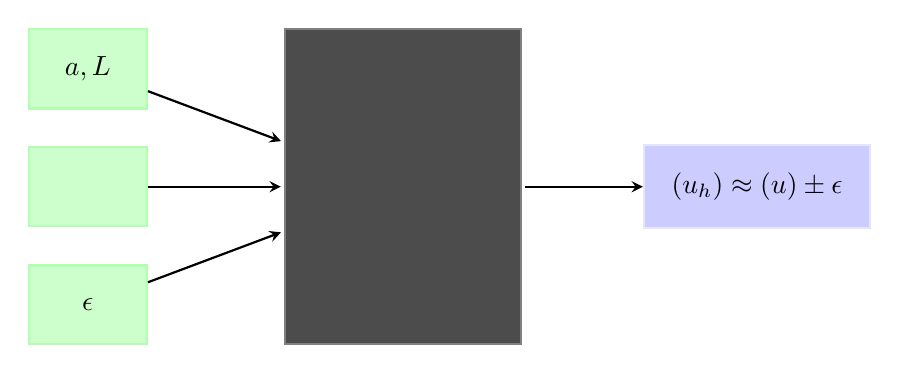
\begin{tikzpicture}[bend angle=45, scale=.8]
      \node[process] (process) {};
      \node[input, node distance=4cm] (input goal) [left of=process]  {$\goal$}
      edge [into] (process);
      \node[input, node distance=1.5cm] (input eq) [above of=input goal]  {$a, L$}
      edge [into] (process);
      \node[input, node distance=1.5cm] (input tol) [below of=input goal]  {$\epsilon$}
      edge [into] (process);
      \node[output, node distance=4.5cm] (output) [right of=process]  {$\goal(u_h) \approx \goal(u) \pm \epsilon$}
      edge [outof] (process);
    \end{tikzpicture}


  \end{center}
  \begin{block}{FEniCS/DOLFIN}
    \vspace{-1em}
    \begin{python}
pde = VariationalProblem(a, L, bc)
pde.solve(u, tol, M)
    \end{python}
  \end{block}
\end{frame}
